\section{Description}

The following paragraphs name and explain all components of the HT500.3 to give you an exact overview. The terms are used consistently throughout this manual and will help you identify any part you may wish to find or order as a spare part. 



\subsection{Functional principle}

The HT500.3 3D Printer uses the \emph{F}used \emph{F}ilament \emph{F}abrication (FFF) process to build up workpieces in subsequent layers of 0.10 to 0.60mm thickness. The plastic filament is heated in the nozzle to its melting temperature and continuously conveyed by a cogwheel. The molten plastic is pressed through the bore of the nozzle tip and onto the heated print bed. After each layer the print bed is lowered by the preset layer height and the next layer is applied. The heat of the newly applied plastic ensures an adequate binding of the layers.

All temperatures and movement commands are provided by the GCODE, a file format previously generated with a \dq slicing\dq software. This file contains all information for a single print job and is uploaded to the 3D Printer via the web interface.

After the workpiece has been finished the user can leave it in the heated build chamber to slowly cool down thus reducing shrinkage and internal tensions, or he can immediately remove it and start the next print job. The layered building process enables the user to create even complex forms that otherwise could not be realized. 

\begin{figure}[H]
  \centering
  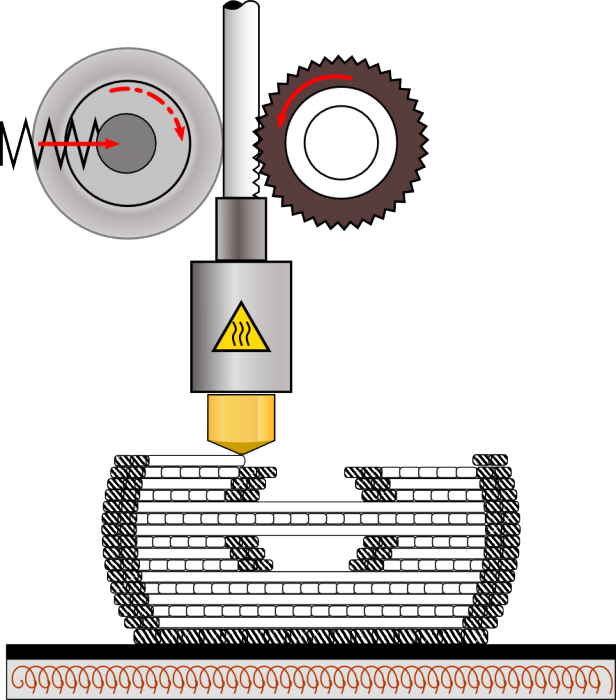
\includegraphics[width=.7\linewidth]{./img/fff_principle_manual.png}
  \caption{The layer-by-layer build-up of random geometries becomes possible with FFF-3D Printers.}
\end{figure}



\subsection{Hardware components}

The HT500.3 is built on an aluminum framework covered with acrylic panels. Its main functional sections are the upper build chamber and the lower electronic chamber. The build chamber is covered with translucent plates to provide insight during production. It contains all mechanical components. At the back cover, the filament supply is installed.

The lower chamber is covered with opaque sheets and contains the electronic components and the mains adapter. All connections and the power switches are located here and the touchscreen for operation is mounted at the front cover.

All covers are fixed to the frame with M4x20 hexagon socket screws and hammerhead nuts, thus being easy to remove and making all around access possible to all parts if required. 

\begin{figure}[H]
  \centering
  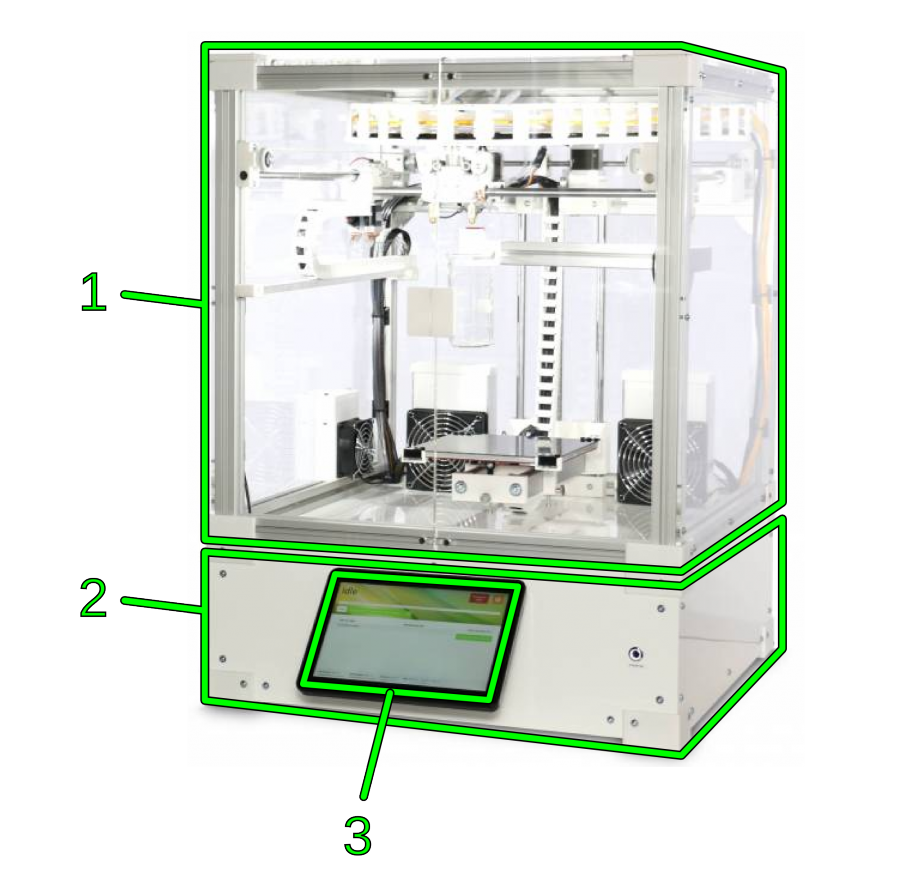
\includegraphics[width=.7\linewidth]{./img/desc_main_1.png}
  \caption{General overview of the HT500.3 3D Printer.}
\end{figure}

\begin{table}[H]
  \centering
  \begin{tabulary}{\textwidth}{ L L }
    \toprule
    No.   &   Description  \\
    \midrule
      1     & Build chamber \\
      2     & Electronic chamber \\
      3     & Touchscreen  \\
    \bottomrule
  \end{tabulary}
\end{table}

All references concerning directions are defined throughout this manual as follows:

\begin{figure}[H]
  \centering
  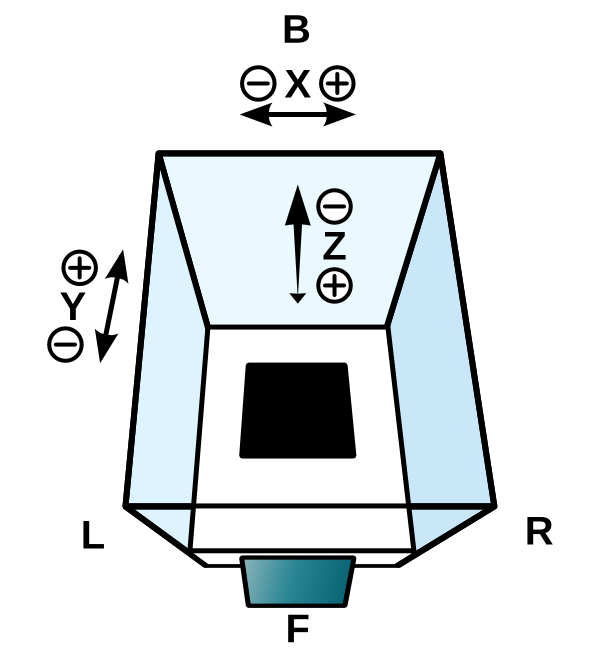
\includegraphics[width=.7\linewidth]{./img/directions_ht500.png}
  \caption{Directions and aspects of the 3D Printer. All statements refer to the frontal view.}
\end{figure}

\begin{table}[H]
  \centering
  \begin{tabulary}{\textwidth}{ L L L }
    \toprule
    Tag      & 	Aspect     &	Description \\
    \midrule
      F 	   &  Front      &	Standing in front of the 3D Printer's touchscreen and looking inside the build chamber. 
                              This is the reference view for all other directions.\\
      L      &	Left       &	Left side of the 3D Printer, referred to the frontal view.\\
      R 	   &  Right      &	Right side of the 3D Printer, referred to the frontal view.\\
      B      &	Back       &	Backside of the 3D Printer, referred to the frontal view.\\ 
    \bottomrule
  \end{tabulary}
\end{table}

All movement directions of the axes are defined throughout this manual as follows: 

\begin{table}[H]
  \centering
  \begin{tabulary}{\textwidth}{ L L L }
    \toprule
    Tag                & 	Called &  	Movement direction \\
    \midrule
    X \textcircled{+}  & 	X positive  &  	Extruder head moves to the right.\\
    X \textcircled{-}  & 	X negative  & 	Extruder head moves to the left.\\
    Y \textcircled{+}  &  Y positive  & 	Extruder head moves backwards.\\
    Y \textcircled{-}  & 	Y negative  & 	Extruder head moves forward.\\
    Z \textcircled{+}  & 	Z positive  &  	Print table moves down.\\
    Z \textcircled{-}  & 	Z negative  & 	Print table moves up. \\
    \bottomrule
  \end{tabulary}
\end{table}

All movements of the extruder drives are defined throughout this manual as follows: 

\begin{figure}[H]
  \centering
  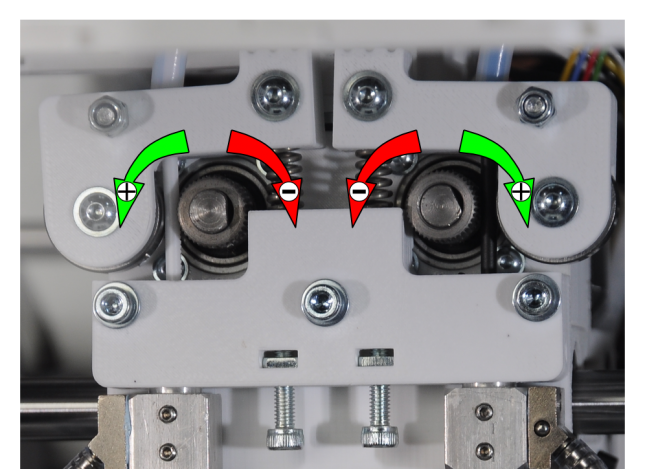
\includegraphics[width=.7\linewidth]{./img/desc_moving_drives.png}
  \caption{Movement directions of the extruder drives.}
\end{figure}

\begin{table}[H]
  \centering
  \begin{tabulary}{\textwidth}{ L L L }
    \toprule
    Tag             &   Called      & Movement direction \\
    \midrule
    \textcircled{+} &	extrude     & Left extruder $\rightarrow$ counter-clockwise rotation\\
                    &               & Right extruder $\rightarrow$ clockwise rotation\\
    \textcircled{-} &	retract     & Left extruder$\rightarrow$ clockwise rotation \\
                    &               & Right extruder $\rightarrow$ counter-clockwise rotation \\
    \bottomrule
  \end{tabulary}
\end{table}


\subsubsection{Build chamber}

\begin{figure}[H]
  \centering
  \includegraphics[width=.7\linewidth]{./img/desc_buildchamber_insideview.png}
  \caption{Inside view of the build chamber.}
\end{figure}

\begin{table}[H]
  \centering
  \begin{tabulary}{\textwidth}{ L L }
    \toprule
    No.  & 	Description \\
    \midrule
      1  & 	Extruder head \\
      2  & 	Print table \\
      3  & 	Heating elements (covered) and fans \\
    \bottomrule
  \end{tabulary}
\end{table}

The build chamber is the main production area with a vertically moving print table and a two-directional horizontally moving extruder head inside.
All electrical motors are installed at their working point and equipped with a water cooling system. The extruder head moves on an H-frame, tooth-belt-driven by two separate stepper motors in X- and Y-direction. The print table is lifted and lowered in Z-direction by a spindle drive.
For regulating the temperature inside the build chamber two heating resistors in separate housings heat the air which then is circulated through the chamber by the fans.
Cables and hoses are installed in and guided by cable carriers.
The access to the build chamber is the magnetically closed double door at the front. 

\begin{figure}[H]
  \centering
  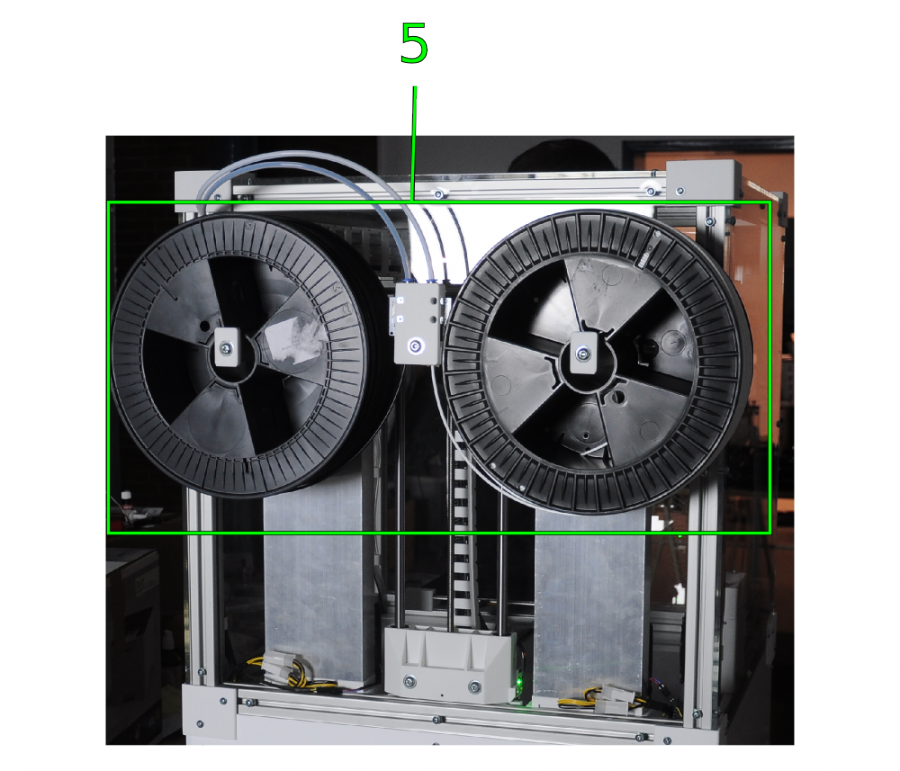
\includegraphics[width=.7\linewidth]{./img/desc_buildchamber_backview.png}
  \caption{Filament supply unit at the rear side of the build chamber.}
\end{figure}

\begin{table}[H]
  \centering
  \begin{tabulary}{\textwidth}{ L L }
    \toprule
    No.  & 	Description \\
    \midrule
      5  &	Filament supply \\
    \bottomrule
  \end{tabulary}
\end{table}

The filament spools that provide the necessary material are installed at the rear of the build chamber next to the filament feed unit.

\subsubsection{Print head components}

\begin{figure}[H]
  \centering
  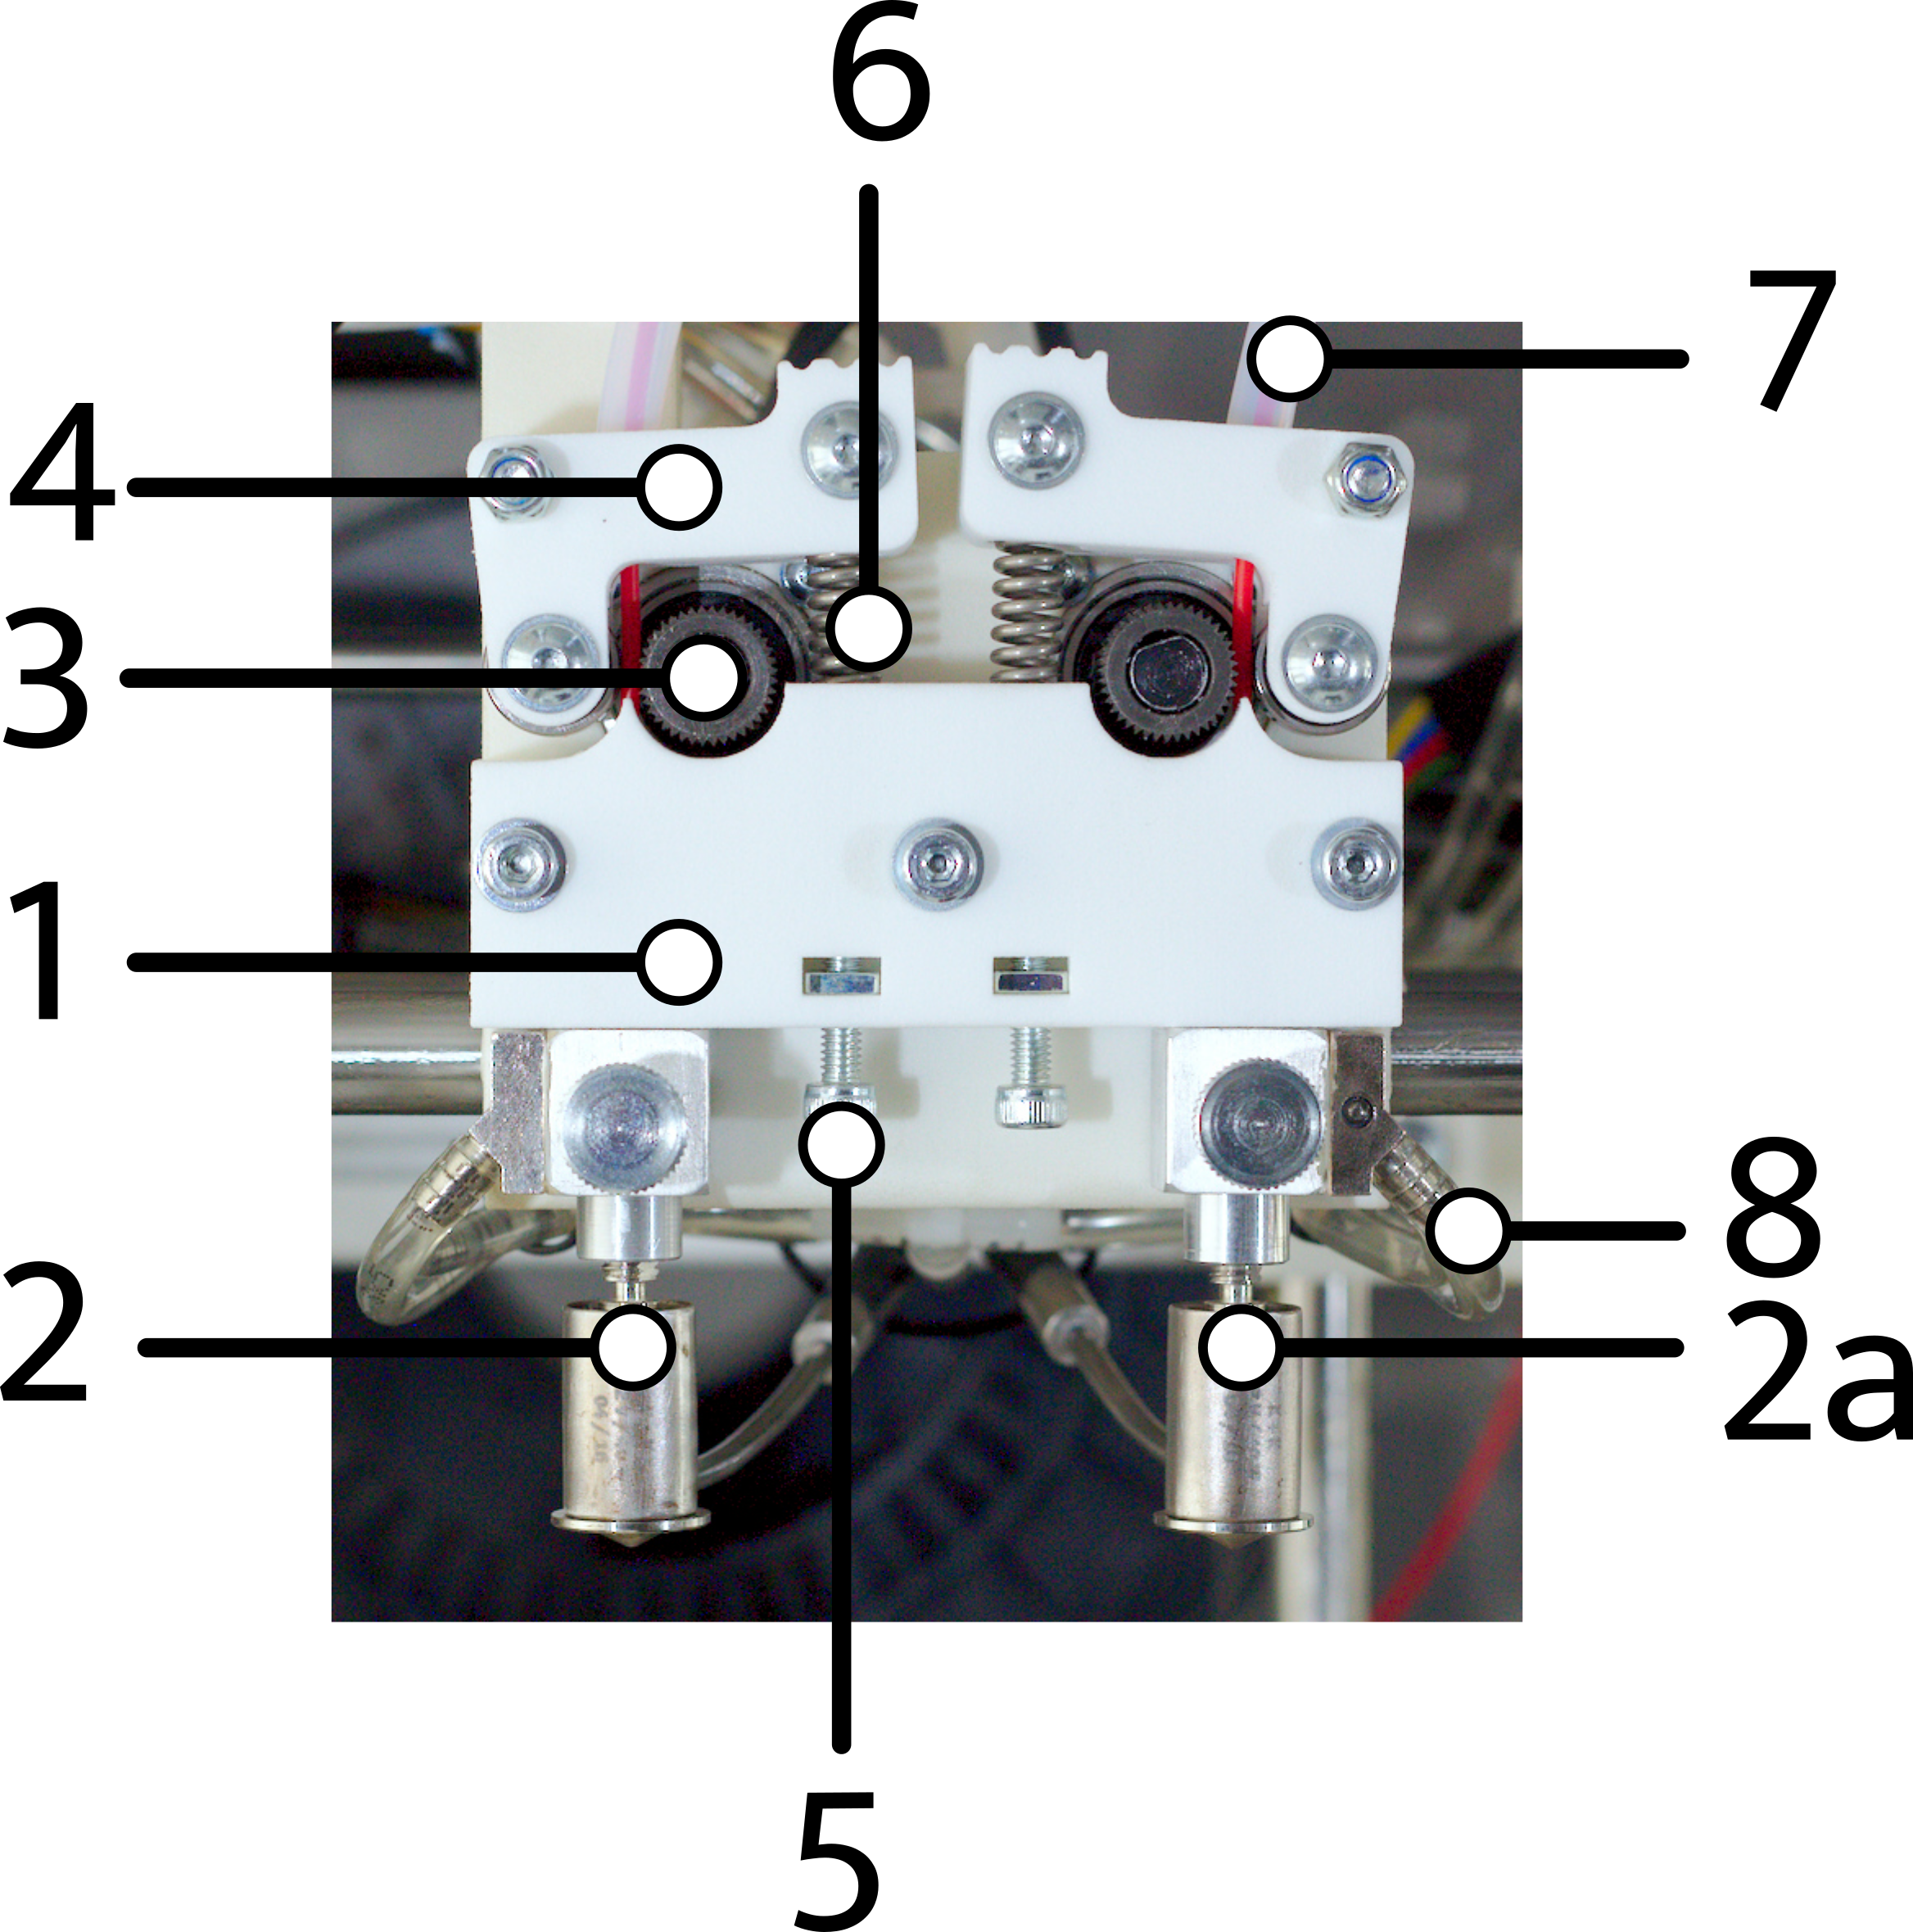
\includegraphics[width=.7\linewidth]{./img/desc_extruderhead.png}
  \caption{Extruder head components}
\end{figure}

\begin{table}[H]
  \centering
  \begin{tabulary}{\textwidth}{ L L }
    \toprule
    No.  & 	Description \\
    \midrule
      1  &	Carriage \\
      2  &  Left (primary) hot end \\
      2a &	Right (secondary) hot end \\
       3 &	Filament drive gear \\
       4 &	Idler lever (release function)\\
       5 &	Spring tensioning screw M4x20 \\
       6 &	Idler spring \\
       7 &	Filament feed hose \\
       8 &	Cooling hoses \\
    \bottomrule
  \end{tabulary}
\end{table}

The extruder head is mounted to the traverse of the H-frame and moves horizontally in X- and Y-direction with useful operating ranges of X = 200 mm and Y = 185 mm.
It contains the filament drive gears forwarding the filament strands and the hot ends which melt and dose the material onto the print table. The filament is supplied through a hose from the filament supply and is clamped between the idler lever and the filament drive gear. The filament drive gear is rotated by the filament feed motor and thereby forwarding the filament strand.
Each hot end is provided with its own filament strand, thus enabling bicolored prints, printing two materials or two objects simultaneously or printing with different extrusion thicknesses (e.g. for outer contours and inner filling structures).

\begin{figure}[H]
  \centering
  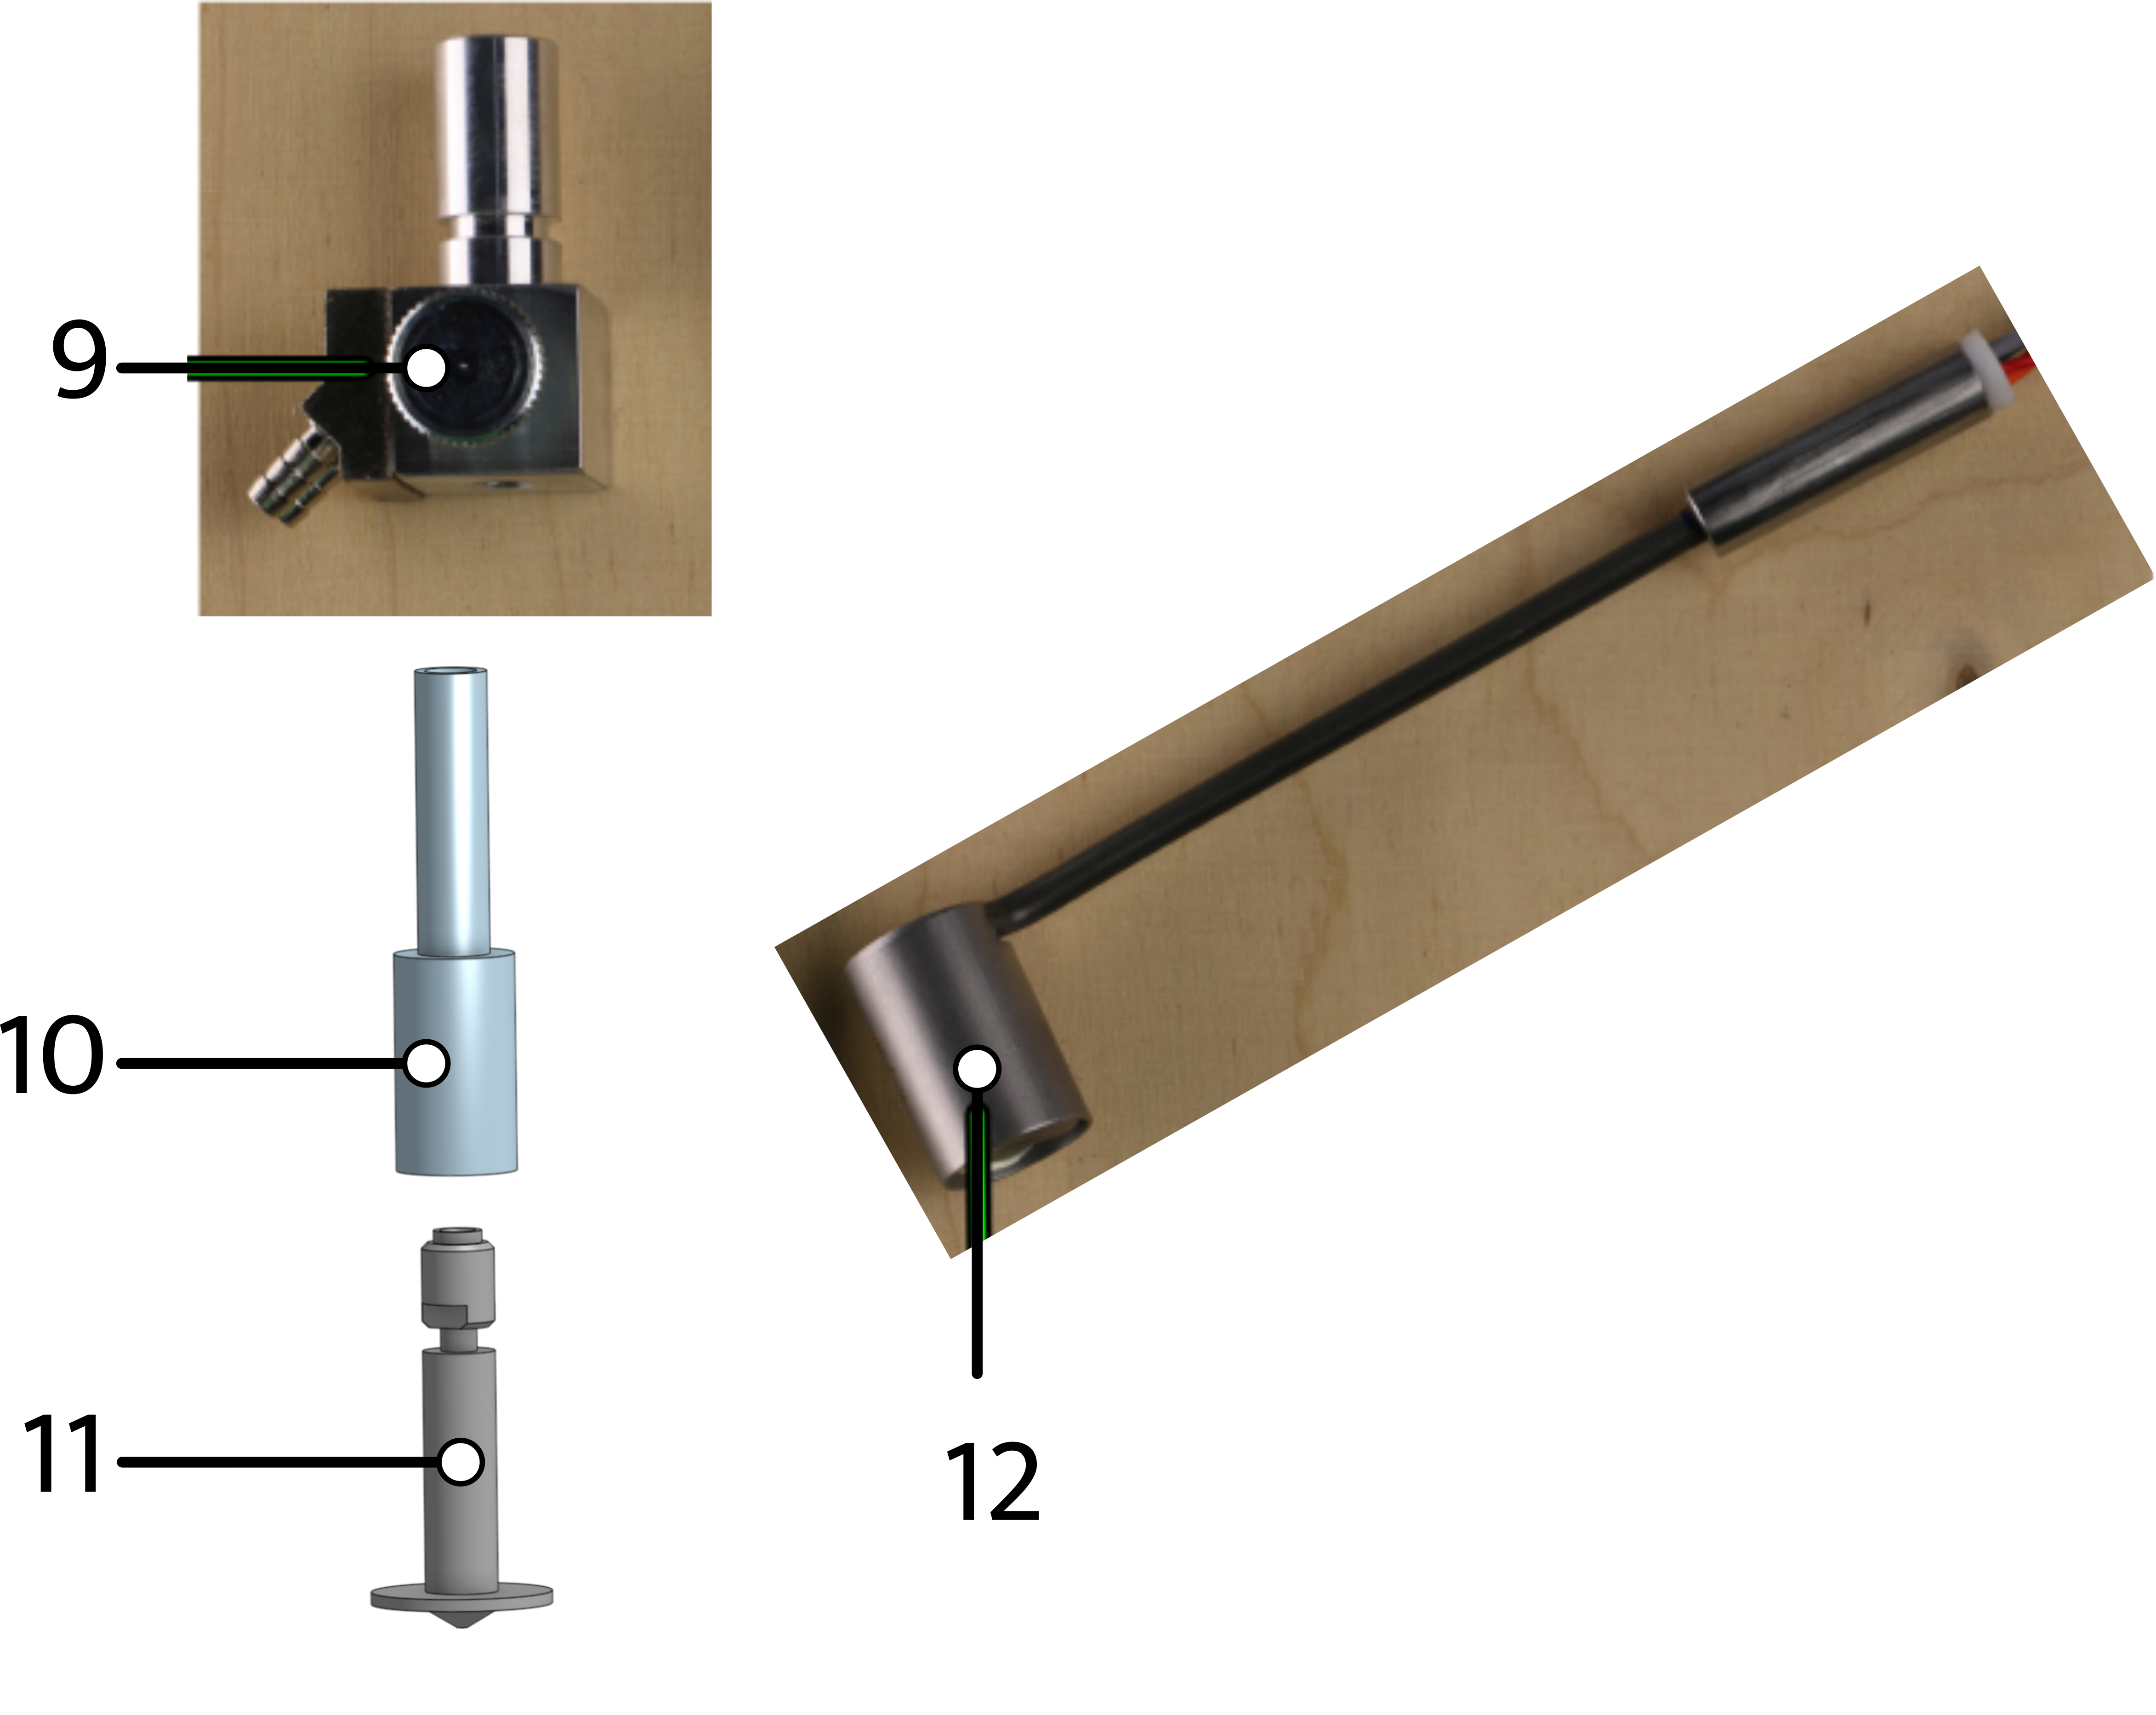
\includegraphics[width=.7\linewidth]{./img/desc_extruderheadcomponents.png}
  \caption{Extruder head components}
\end{figure}

\begin{table}[H]
  \centering
  \begin{tabulary}{\textwidth}{ L L }
    \toprule
    No.  & 	Description \\
    \midrule
     9 &	Aluminum hot-end mount (cooling block) with thumb screw and cooling hose adapter\\
    10 &	Nozzle Adapter\\
    11 &	Nozzle\\
    12 &	500\degree C heating cartridge with integrated thermocouple\\
    \bottomrule
  \end{tabulary}
\end{table}

Each hot-end is heated by a ceramic heating cartridge so that the filament is molten inside the nozzle. The integrated thermocouple provides direct alignment of set and actual temperature.
To improve the thermal control of the melting process the hot-end mount is connected to the cooling system, ensuring an even temperature distribution in a well defined area of the nozzles so that there is a preheating zone and a melting zone. 

\begin{figure}[H]
  \centering
  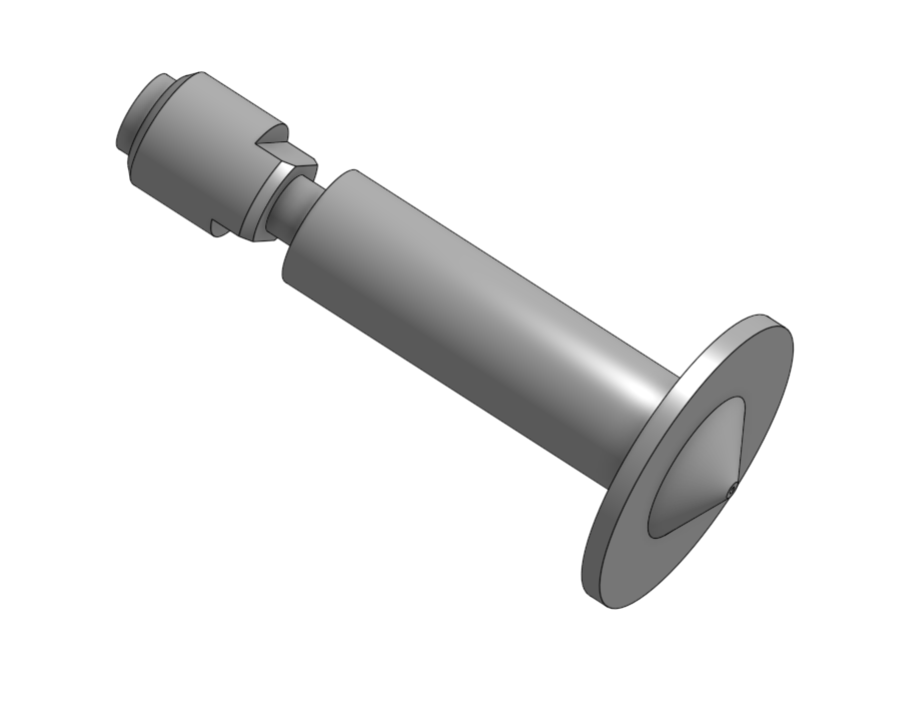
\includegraphics[width=.7\linewidth]{./img/desc_nozzle.png}
  \caption{A single nozzle.}
\end{figure}

The nozzle is exchangeable to provide different bore diameters for different materials, layer thicknesses or print speed. Ex factory, the 0.35mm tip is preinstalled on the left extruder and 0.5mm on the right extruder. Additionally, 0.75mm nozzles are available

\subsubsection{Print table and print bed}

The print table is mounted on the crossbeams of the elevator assembly which is positioned in Z-direction in its useful operating range by a spindle drive.

The print table itself consists of an aluminum sandwich panel with a silicone rubber heating pad, providing an even temperature distribution and ensuring optimal adhesion throughout the printing process. 

\begin{figure}[H]
  \centering
  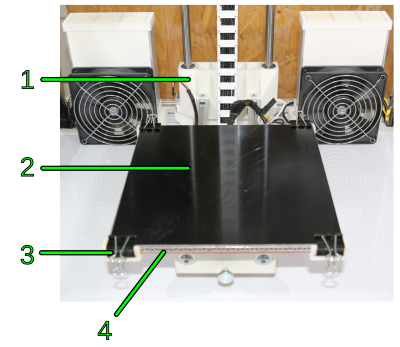
\includegraphics[width=.7\linewidth]{./img/print_table_overview.png}
  \caption{Print table and print bed fastened with four bulldog clamps}
\end{figure}

\begin{table}[H]
  \centering
  \begin{tabulary}{\textwidth}{ L L }
    \toprule
    No.  &  Description \\
    \midrule  
      1  &  Elevator assembly \\
      2  &  Removable PEI/ Carbon Fiber print bed \\
      3  &  Bulldog clamp \\
      4  &  Heated print table \\
    \bottomrule
  \end{tabulary}
\end{table}

It rests on three springs lockable with set screws for an even and accurate leveling since a precisely adjusted distance between print bed and nozzle tip is vital for the print bed adhesion an the print results.

The semi-automated leveling process is described in the Operating Manual.

Print jobs are executed on the removable print bed laid on the print table and fixed with four bulldog clamps at the corners. This fixation allows the use of print beds of different thicknesses.
The standard print bed included in the delivery is a 210x210x1.8mm polyetherimide (PEI) carbon fabric plate that provides excellent adhesion for a large variety of materials, including ABS, Nylon, PET, PC, HIPS, TPU and other. 

\begin{figure}[H]
  \centering
  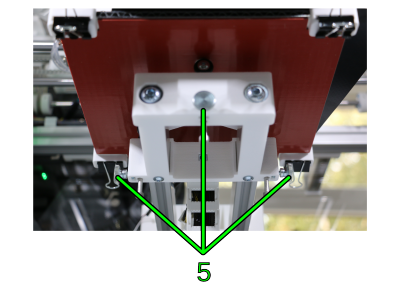
\includegraphics[width=.7\linewidth]{./img/print_table_overview_2.png}
  \caption{3-point leveling support}
\end{figure}

\begin{table}[H]
  \centering
  \begin{tabulary}{\textwidth}{ L L }
    \toprule
    No.  &  Description \\
    \midrule  
      5  &  Set screws of the spring-mounted 3-point leveling support \\
    \bottomrule
  \end{tabulary}
\end{table}

\paragraph{Important print bed knowledge}

The PEI carbon fabric composite print beds are, in accordance with the HT500.3's standards, optimized for printing ABS and are custom-made to Kühling\&Kühling specifications. It also works fine with HIPS, PET-Copolyester, PVA and thermoplastic urethane (TPE-U). Other materials may require a different subsurface, be it another material or a special treatment with tape or glue.

PEI is highly resistant to a lot of solvents which makes it a suitable subsurface for a lot of materials since removing residues and refurbishing for the next print becomes quite easy.

Find more information about the Kühling\&Kühling PEI print bed:

\begin{itemize}
  \item Operating and handling are described in the Operating manual.
  \item Cleaning and care can be found in the Service guide.
\end{itemize}


\subsubsection{Drives}

\begin{table}[H]
  \centering
  \begin{tabulary}{\textwidth}{ L L }
    \toprule
    No.  & 	Description \\
    \midrule  
    1    &	X-axis motor (extruder head motor) \\
    2    &	Y-axis motor (H-frame traverse motor) \\
    3    &	Z-axis motor (spindle drive of print table) \\
    4    &	Filament feed motors (filament gear drive) \\
    \bottomrule
  \end{tabulary}
\end{table}

Five electrical stepper motors, one per direction of the extruder head, one for lifting and lowering the print table and one per extruder head nozzle for forwarding the filament, provide all necessary movement for printing. All motors are equipped with water cooling to prevent overheating due to workload and the heating of the build chamber.

\begin{figure}[H]
  \centering
  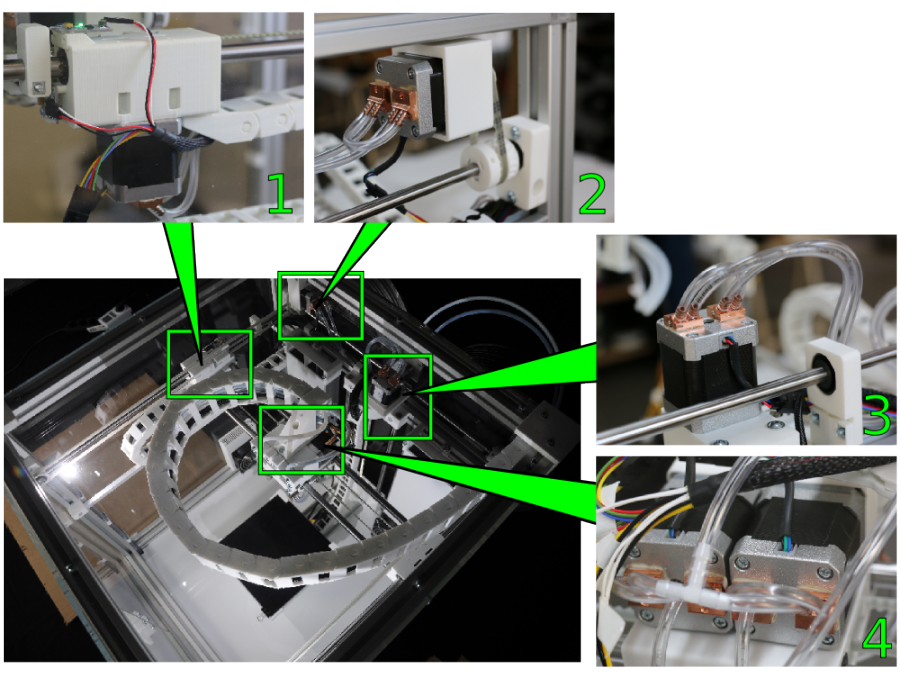
\includegraphics[width=.7\linewidth]{./img/desc_drives_2.png}
  \caption{Single views of the drive motors.}
\end{figure}


\subsubsection{Sensors}

Sensors for positioning and temperature control are installed inside the build chamber.

Every axis is equipped with a Hall effect sensor and a magnet for accurate home positioning. If the Hall effect sensor nears the magnet and measures the defined threshold value of the magnetic field strength, the sensor effects a \dq stop\dq signal via the machine controller. After all sensors have given this signal the moving axes are in home position. The home position is the reference value for all relative movement of the extruder head and the print bed.

\begin{figure}[H]
  \centering
  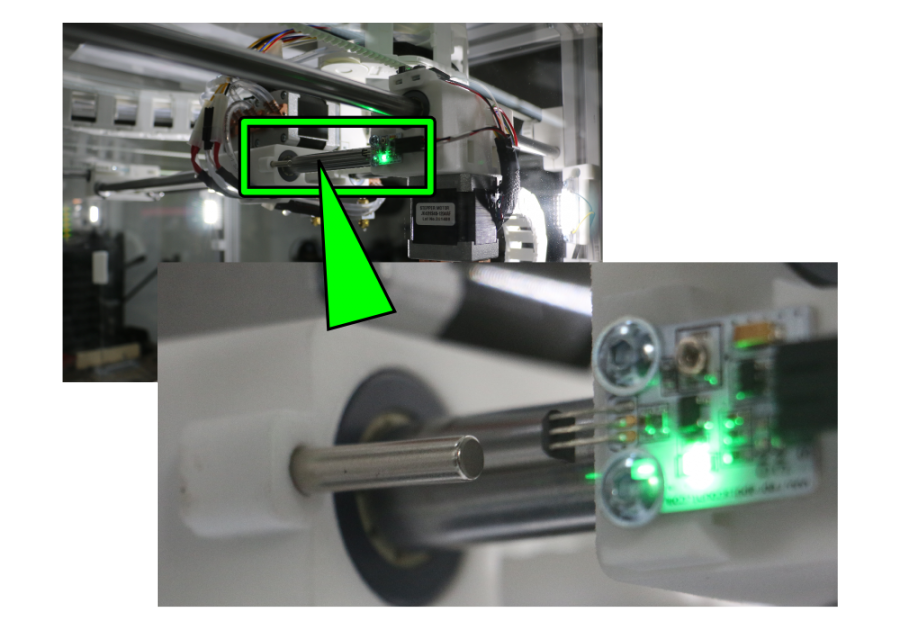
\includegraphics[width=.7\linewidth]{./img/desc_x-sensor.png}
  \caption{Hall effect sensor and magnet of the X-axis.}
\end{figure}

\begin{figure}[H]
  \centering
  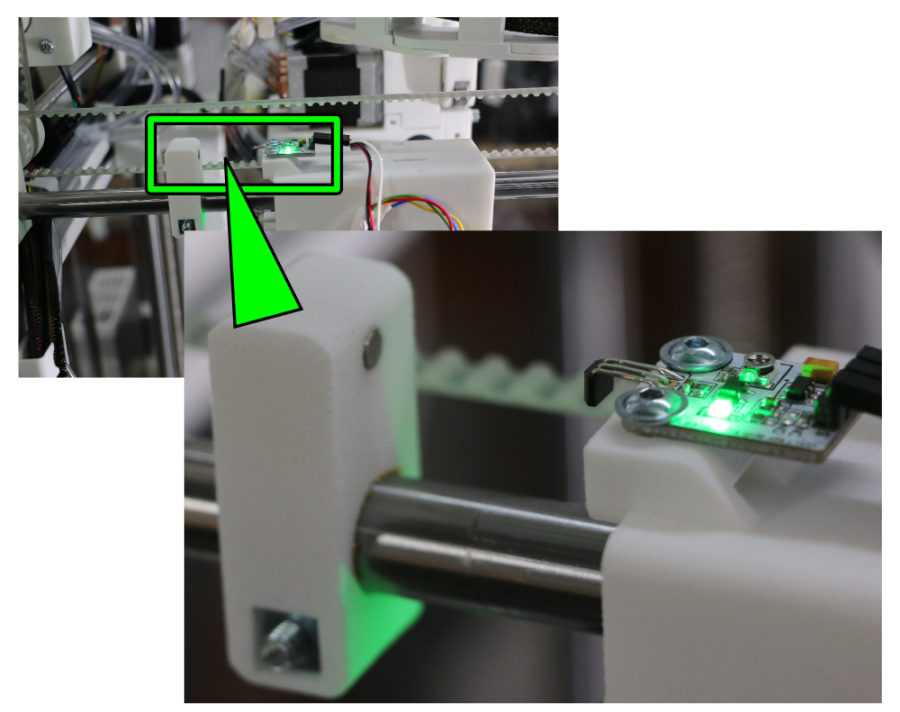
\includegraphics[width=.7\linewidth]{./img/desc_y-sensor.png}
  \caption{Hall effect sensor and magnet of the Y-axis.}
\end{figure}

\begin{figure}[H]
  \centering
  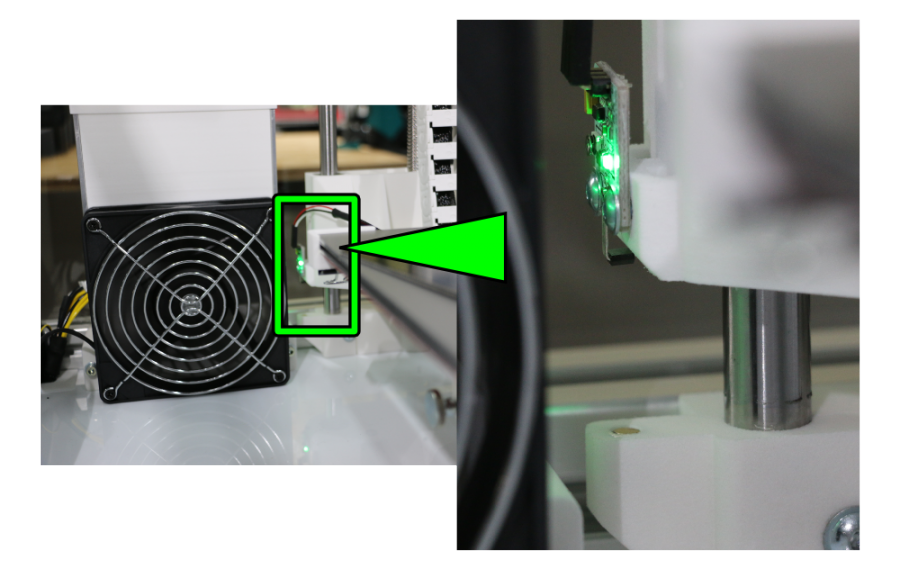
\includegraphics[width=.7\linewidth]{./img/desc_z-sensor.png}
  \caption{Hall effect sensor and magnet of the Z-axis.}
\end{figure}

Thermistors measure the relevant temperatures for the printing process, i.e. the print bed temperature and the build chamber temperature. 
All thermistors deliver their input signal to the machine controller and thus effect switching on and off the according heating resistor.

The print bed temperature is measured directly at the heating pad with which it is looped in a control circuit.
The build chamber sensor is installed at the elevator assembly and measures the air temperature inside the build chamber. Its measurements influence the control of the heating resistors inside the heating elements.

The extrusion temperature is measured directly at the heating cartridge by an integrated thermocouple.

\begin{figure}[H]
  \centering
  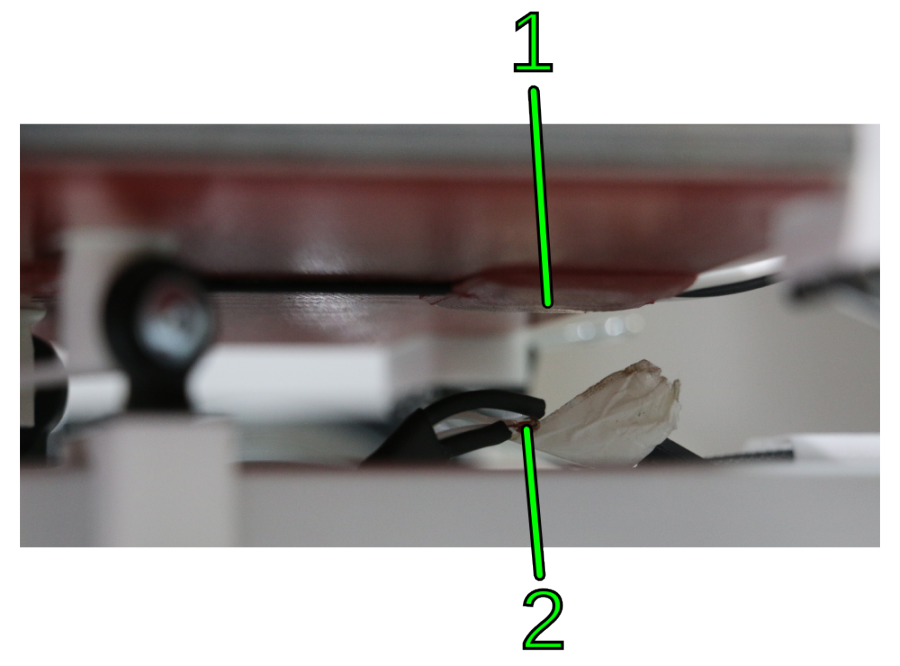
\includegraphics[width=.7\linewidth]{./img/desc_thermistors_printbed_chamber.png}
  \caption{Thermistors of the print bed (1) and the build chamber (2)}
\end{figure}

A limit switch is installed at every filament inlet of the filament feed unit
(see below). 


\subsubsection{Filament supply}

\begin{table}[H]
  \centering
  \begin{tabulary}{\textwidth}{ L L }
    \toprule
    No.  & 	Description \\
    \midrule  
    1    & 	Feed unit \\
    2    & 	Filament spool carrier \\
         & 	Filament spool (2.3 kg) \\
    4    & 	Limit switch \\
    5    & 	Filament inlet with dust wiping sponge \\
    \bottomrule
  \end{tabulary}
\end{table}

The HT500.3 is designed for printing filament strands of a diameter of 1.75 mm with a tolerance of $\pm$ 0.05 mm.
Two separate strands can be fed from the outside to the extruder head. One filament spool can be positioned on each spool carrier; a stop collar prevents them from falling off due to their rotation.
The end of the filament strand is manually inserted into the inlet of the feed unit and led through hoses to the two extruder nozzles. At the inlet the filament is put through a sponge that wipes dust off the strand to keep the material unsoiled before reaching the nozzle.
A limit switch registers the end of the filament strand when the spool is empty. The print process then is interrupted and the lack of material is signaled on the touchscreen. The printing process can be resumed after refilling the supply. 

\begin{figure}[H]
  \centering
  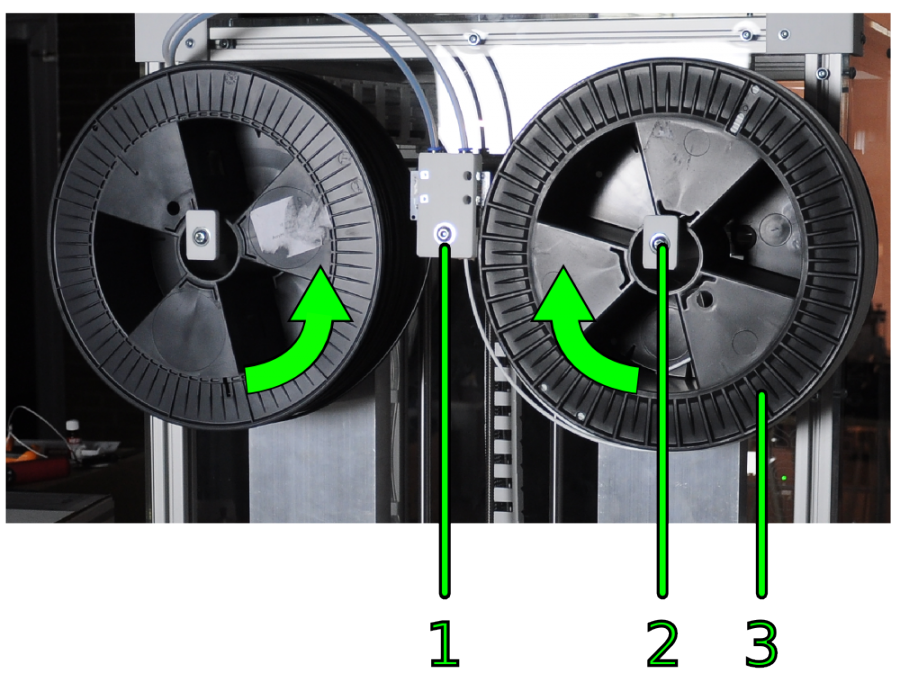
\includegraphics[width=.7\linewidth]{./img/desc_filamentfeedunit.png}
  \caption{Filament supply}
\end{figure}


\begin{figure}[H]
  \centering
  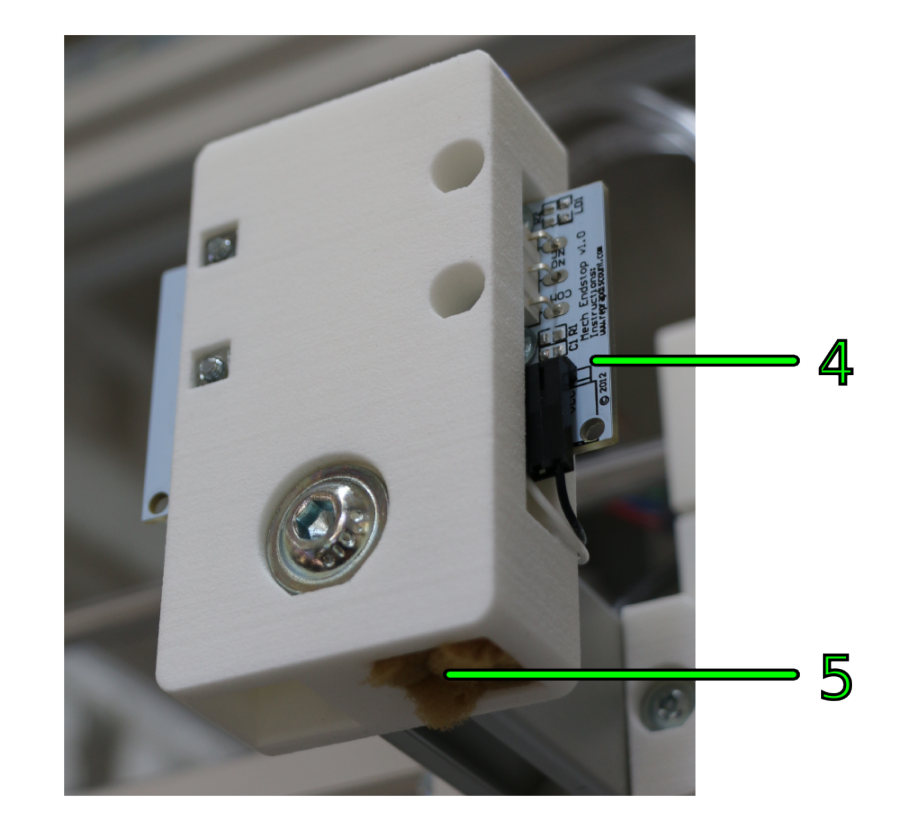
\includegraphics[width=.7\linewidth]{./img/desc_filamentfeedunit_dustsponge.png}
  \caption{Filament inlet with limit switch and dust wiping sponge.}
\end{figure}


\subsubsection{Wiper}

\begin{table}[H]
  \centering
  \begin{tabulary}{\textwidth}{ L L }
    \toprule
    No.  & 	Description \\
    \midrule  
    1    & 	Wiper lip \\
    2    & 	Bracket \\
    3    & 	Excess retainer \\
    4    & 	Mounting arm \\
    \bottomrule
  \end{tabulary}
\end{table}

\begin{figure}[H]
  \centering
  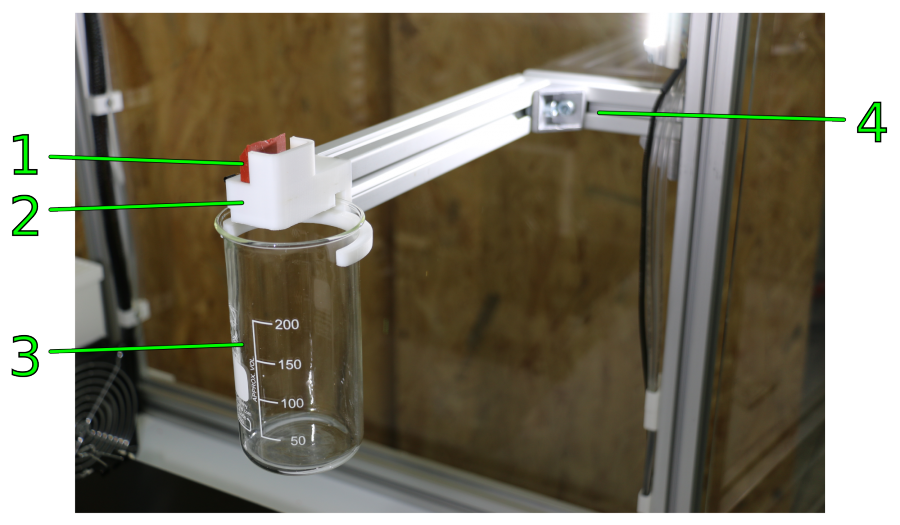
\includegraphics[width=.7\linewidth]{./img/desc_wiper.png}
  \caption{The wiper makes sure that the nozzle tip is always clean and well filled after a tool change during dual-material print jobs.}
\end{figure}

The HT500.3 3D Printer is equipped with a wiper to enable high-quality dual extruder printing.

During every tool change of a dual-extruder print, the nozzle to be used next will be primed and wiped to ensure pressure loss during its pause time is compensated and the nozzle starts well filled. 



\subsection{Electronic chamber}

\begin{figure}[H]
  \centering
  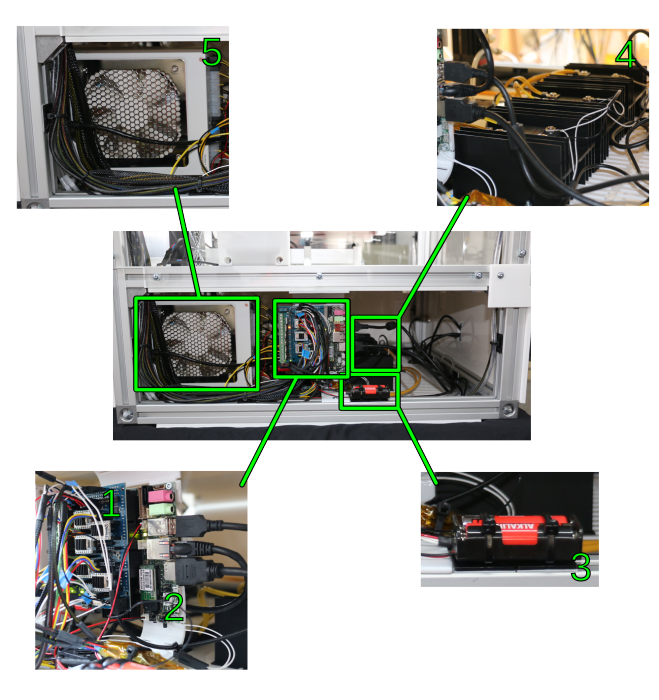
\includegraphics[width=.7\linewidth]{./img/desc_ht-500_overviewelectronicchamberleft.png}
  \caption{Inside view of the electronic chamber (left side).}
\end{figure}

\begin{table}[H]
  \centering
  \begin{tabulary}{\textwidth}{ L L }
    \toprule
    No.  &  Description \\
    \midrule  
    1    &  RADDS v1.5 3D Printer Driver Shield \\
    2    &  UDOO Quad Single Board Mini PC \\
    3    &  3V power supply for internal real-time clock \\
    4    &  Solid State Relays on cooling substructure \\
    \bottomrule
  \end{tabulary}
\end{table}

All control elements are installed in the electronic chamber together with the 12V(DC) mains adapter and the cooling unit.

The chamber is completely covered with white acrylic sheets fastened to the aluminum frame with hexagon socket screws and hammerhead nuts.

The RADDS 3D Printer Driver Shield in conjunction with the SAM3X microcontroller on the UDOO board controls all processes of the printing process, i.e. the drives, the heating resistors, heating fans and the temperature sensors.

The UDOO Quad Single Board Mini PC provides the GUI of the touchscreen and the ethernet connection and processes the G-codes of the slicing software.
Slots in the bottom cover provide an air inlet for the cooling unit.

When the 3D Printer is switched off the internal real-time clock of the Mini PC is fed by two external batteries so that the system's time signal is not lost.

The solid state relays switch the four heating resistors of the build chamber heating and the heating resistor of the print table.

\subsection{Cooling system}

The cooling unit consists of a pump with water reservoir, a radiator and the closed loop coolant circuit filled with an electronic cooling liquid. It is automatically switched on and off when the build chamber is activated/deactivated.

The coolant is pumped in a circle past the motors and the extruder nozzles where it absorbs heat which is then emitted via the radiator.

Check the coolant level monthly and if required, refill as described in the Service Guide. 

\begin{figure}[H]
  \centering
  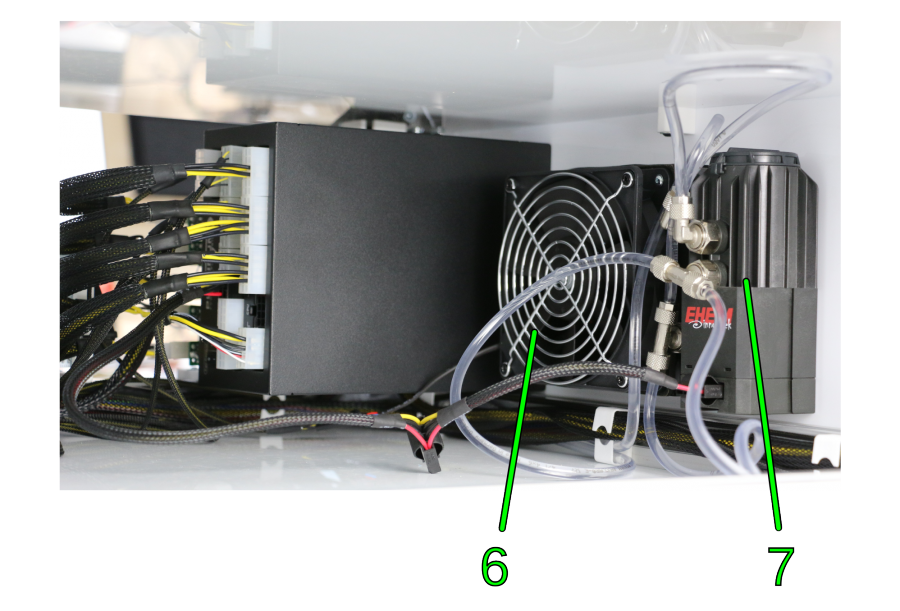
\includegraphics[width=.7\linewidth]{./img/desc_ht500_overviewelectronicchamberright.png}
  \caption{Inside view of the electronic chamber (right side).}
\end{figure}

\begin{table}[H]
  \centering
  \begin{tabulary}{\textwidth}{ L L }
    \toprule
    No.  &  Description \\
    \midrule  
    6    &  Cooling unit radiator \\
    7    &  Cooling unit pump \\
    \bottomrule
  \end{tabulary}
\end{table}

\subsection{Connections and Controls}

\begin{figure}[H]
  \centering
  \includegraphics[width=.7\linewidth]{./img/desc_overviewelectronicchamberhind_typeplate.png}
  \caption{Rear cover}
\end{figure}

\begin{table}[H]
  \centering
  \begin{tabulary}{\textwidth}{ L L }
    \toprule
    No.  &  Description \\
    \midrule
    8    &  Type plate \\
    9    &  Cooling unit water pump and radiator grill \\
    10   &  Mains plug \\
    11   &  Main switch \\ 
    12   &  RJ45 ethernet plug \\
    13   &  230V supply cable with Schuko plug \\
    \bottomrule
  \end{tabulary}
\end{table}

At the rear cover you find the mains plug and the main switch of the mains adapter and the RJ45 ethernet plug for the network connection.

The cooling systems' accumulated warmth is dissipated via the radiator grill to the outside.
The type plate is positioned next to the fixing screws of the cooling water pump. 

\begin{table}[H]
  \centering
  \begin{tabulary}{\textwidth}{ L L }
    \toprule
    No.  & 	Description \\
    \midrule
    14   &	10\textquotedbl TFT high-resolution touchscreen with Graphical User Interface (GUI) \\
    15   &	Wake button \\
    \bottomrule
  \end{tabulary}
\end{table}

\begin{figure}[H]
  \centering
  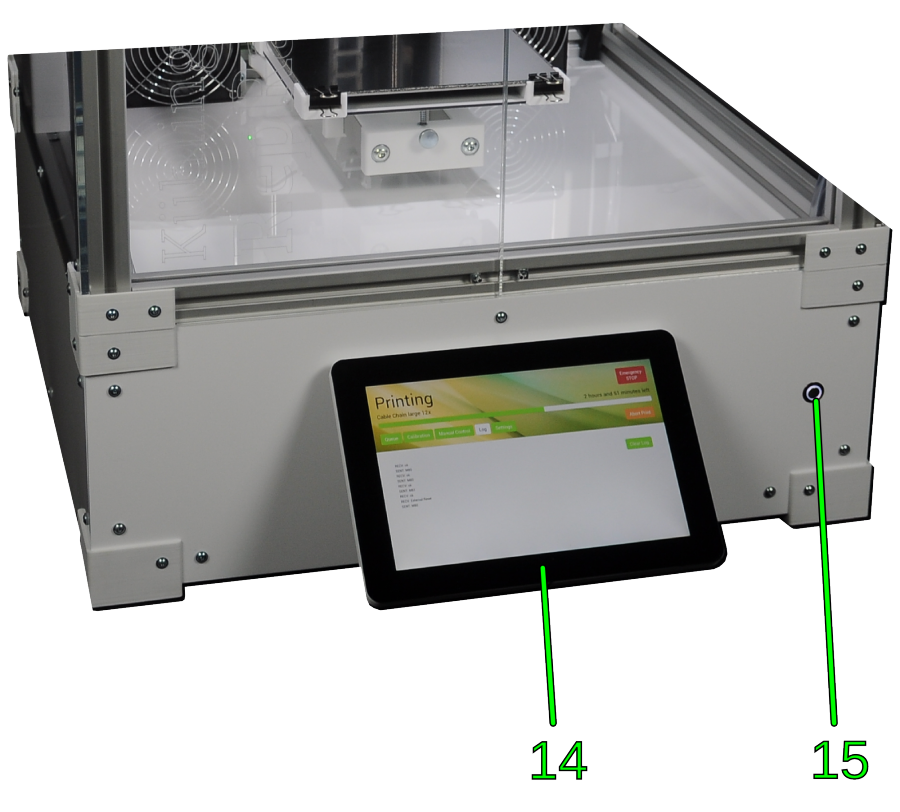
\includegraphics[width=.7\linewidth]{./img/desc_ht500_electronicchamberfront.png}
  \caption{Touchscreen user interface and wake button at the front cover}
\end{figure}

The wake button at the front panel provides a wake-up function and indicates the general operating status of the 3D Printer. It is equipped with a light ring that is illuminated while operational and dims after the 3D Printer has been shut down. Press the button to restart the 3D Printer from standby.

All 3D Printer operation is carried out via the Graphical User Interface at the touchscreen. 



\subsection{Touchscreen operation}

Operating the HT500.3 is designed to be comfortable and intuitive. Therefore, a high-resolution 10\textquotedbl TFT touchscreen mounted at the front panel provides an easy-to-use Graphical User Interface (GUI).

All operation of the HT500.3 is carried out via the RepRapOnRails operating software which provides status messages and control functions that can be chosen by simply tapping the respective buttons. Find detailed explanations of functions and operating procedures in the Operating Manual.

\begin{figure}[H]
  \centering
  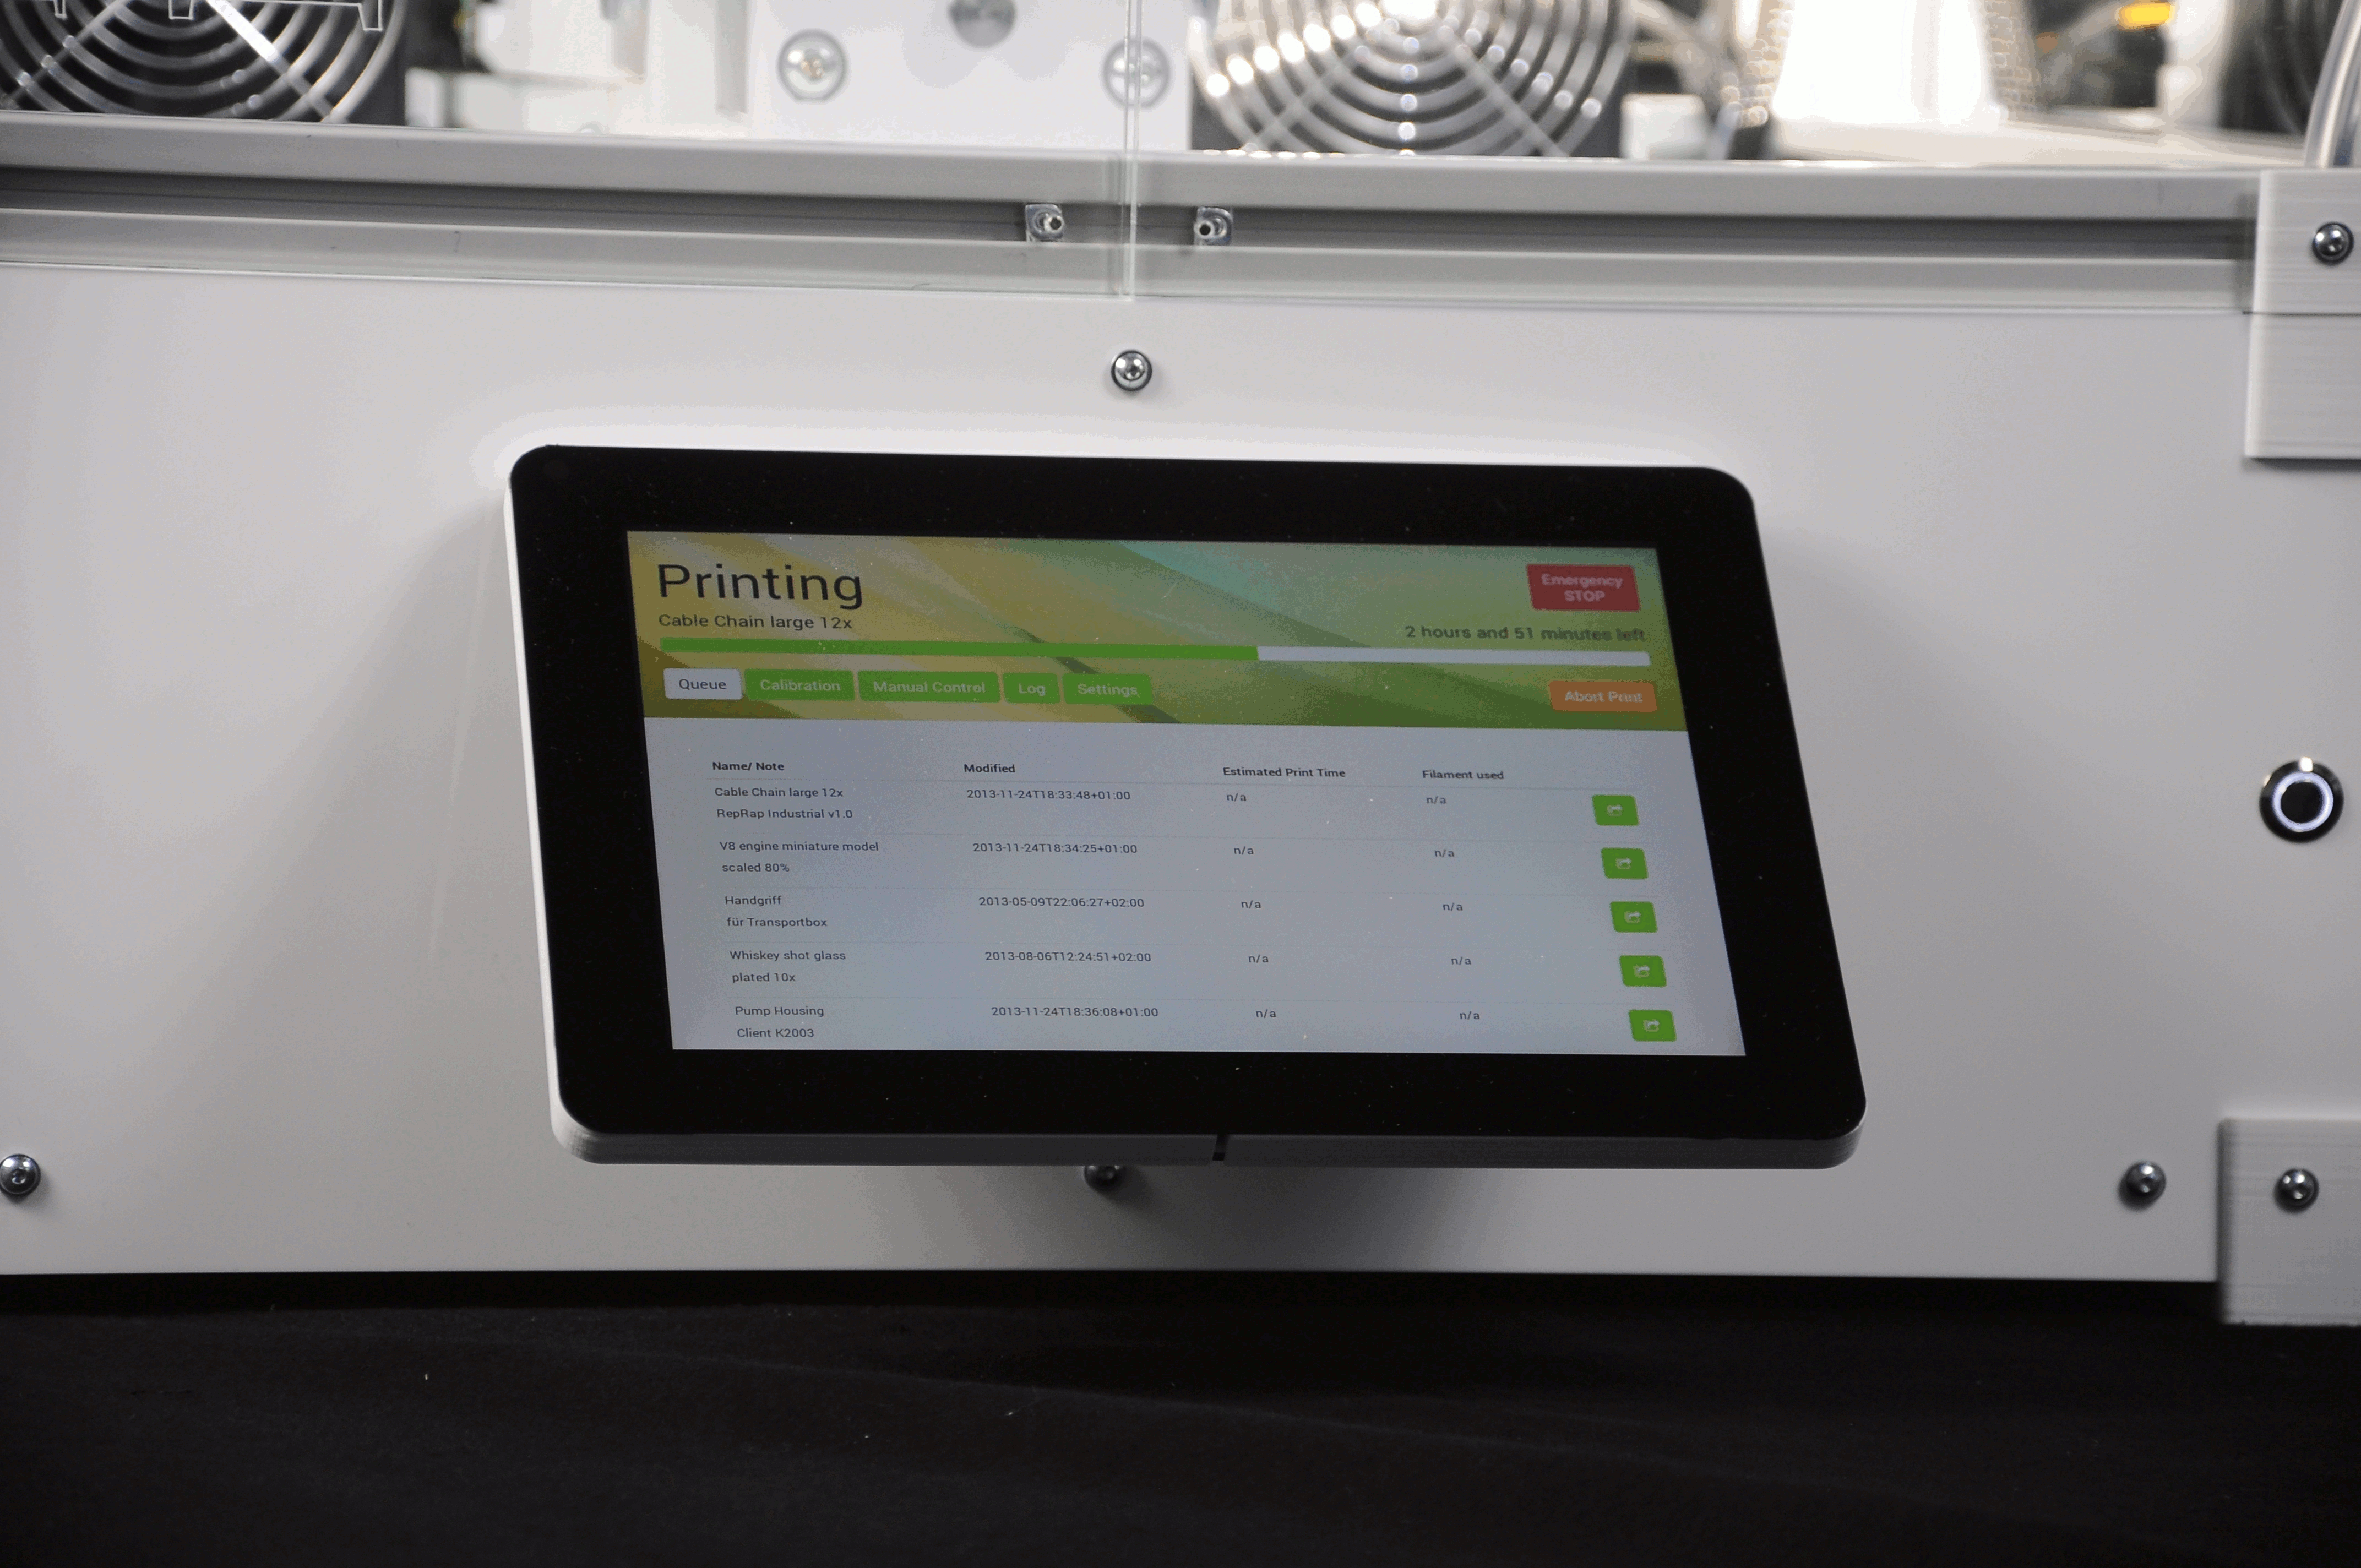
\includegraphics[width=.7\linewidth]{./img/touchscreen.png}
  \caption{The high-resolution 10\textquotedbl-TFT touchscreen mounted at the front panel enables direct operation of the HT500.3.}
\end{figure}

The currently installed version
of the operating software is displayed on the right-hand side of \emph{Setup} menu together with additional system information.

\begin{figure}[H]
  \centering
  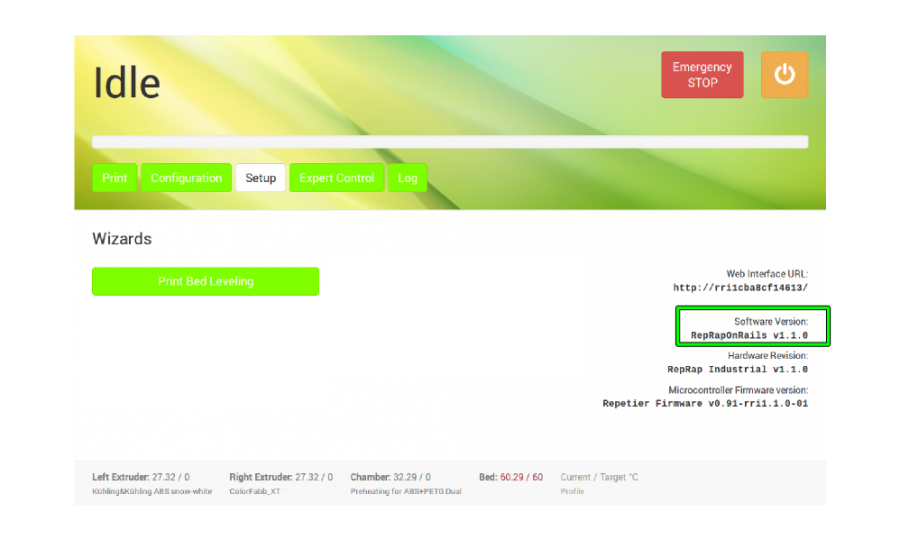
\includegraphics[width=.7\linewidth]{./img/gui_setupmenu_rrorversion.png}
  \caption{RepRapOnRails software version displayed in the \emph{Setup} menu.}
\end{figure}

